\chapter{Layout recognition for tabular data}

The extraction of table structures from a page poses various difficulties. Complications mostly arise when the input document does not correspond to the typical one-column, graphics-free layout. This may cause the spaces between individual page columns to be interpreted as table column spaces, which may lead to the detection of a two-column full page table and a complete rejection of any tables present in page columns. Additionally, complex layouts often cause difficulties when determining the reading order of the document. Therefore, in most cases, a \emph{layout analysis} first needs to performed.

\section{Layout analysis}

\emph{Layout analysis} is the process of identifying and categorizing image document elements, such as figures, tables, forms, math symbols, headers, footers or simple paragraph text (\emph{geometric layout analysis}) and semantically labeling them according to their logical roles (\emph{logical layout analysis}).

In the previous chapter, we already covered the basics of geometric layout analysis, which is the same process as \emph{page segmentation}. The output of this process is a data structure containing the information about the detected elements. Depending on the configuration of the analysis, the resulting elements can be of various types, such as characters, words, text lines, or even tables and forms. A logical layout analysis is the applied on these elements.

\emph{Logical layout analysis} is used to determine the reading order of the image document. It adopts the idea of \emph{labels}, which provide an information about the semantic order and type of individual documents elements. For example, a label might be just a number indicating the reading order of the element (as presented in~\cref{fig:readingOrderExample}), or it could contain more complex information, such as "table header", "page footer", "image caption"\ldots

The result of logical layout analysis is therefore often in a form of mapping of each element to its corresponding label. However, the determination of correct labels is sometimes hard even for human perception, as presented in~\cref{fig:readingOrderProblems}. With various differently aligned columns with different font sizes, or with image captions appearing on different sides of the image in every document, people often determine which elements belong together only according to their intuition (e.g. when reading about a recent earthquake, caption saying “Rescued puppy” probably belongs to the picture of a dog instead of a flooded beach, although in can be placed right in the middle of these two images).

Computers have no notion of such things. This is often a cause of many errors and a reason why a lot of OCR engines claim to work on only documents with specified layouts, e.g. single-column, non-graphical\ldots

\begin{figure}[t]
\centering
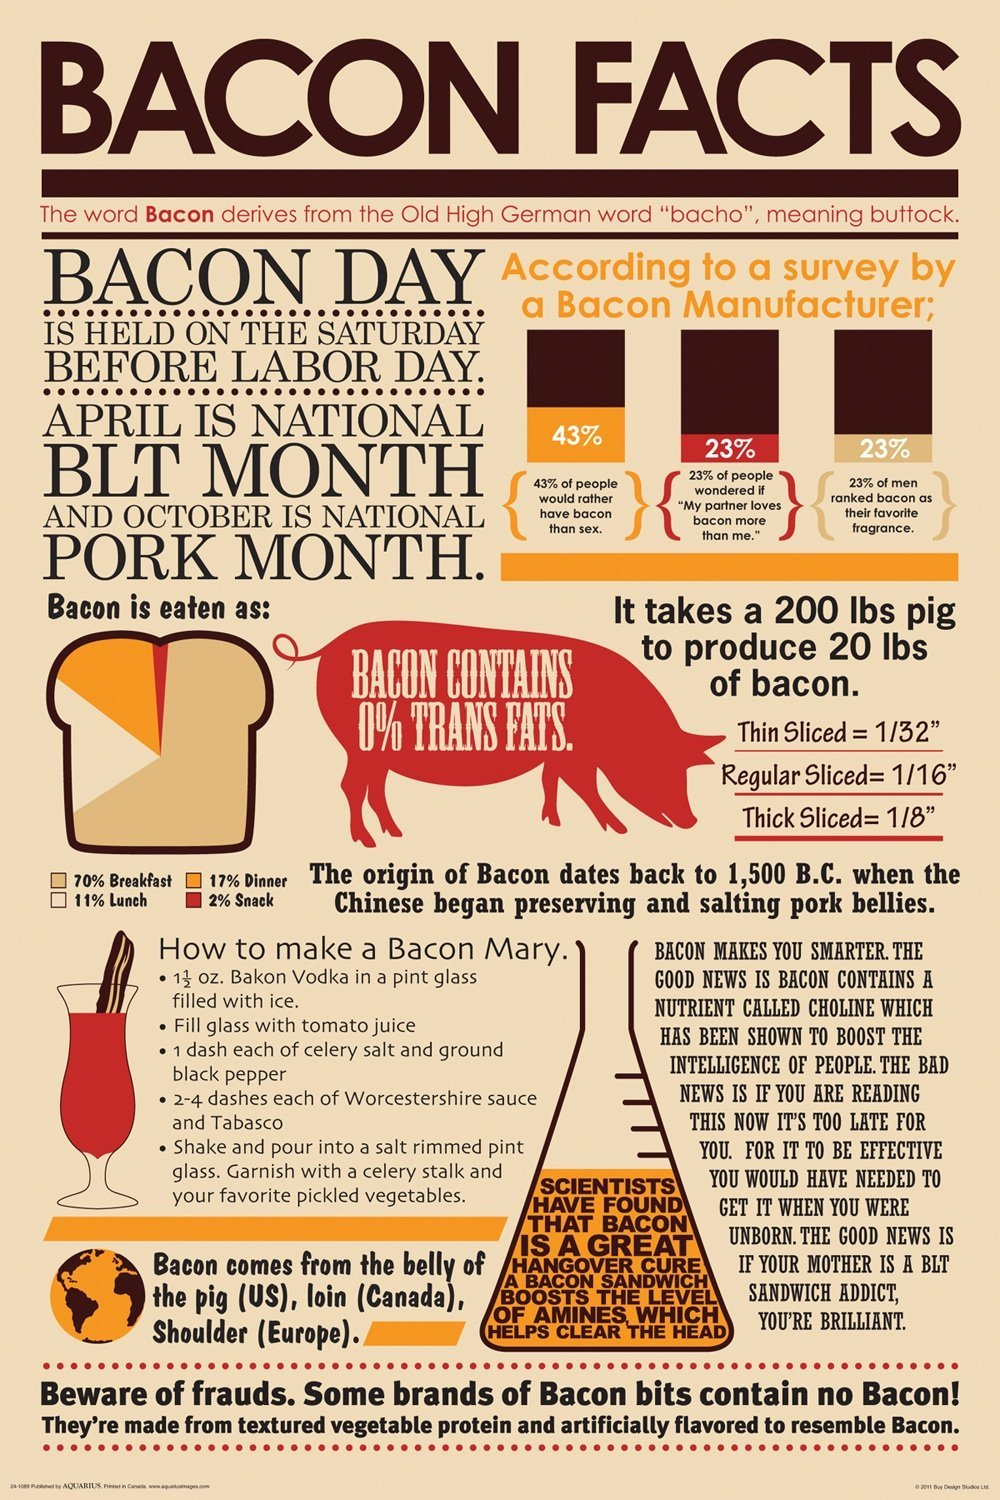
\includegraphics[width=0.5\linewidth]{img/tableDetection/readingOrderIssue.jpg}
\caption{Reading order problems. Determination of correct labels is sometimes hard even for human perception.} \label{fig:readingOrderProblems}
\end{figure}

\begin{figure}[t]
\centering
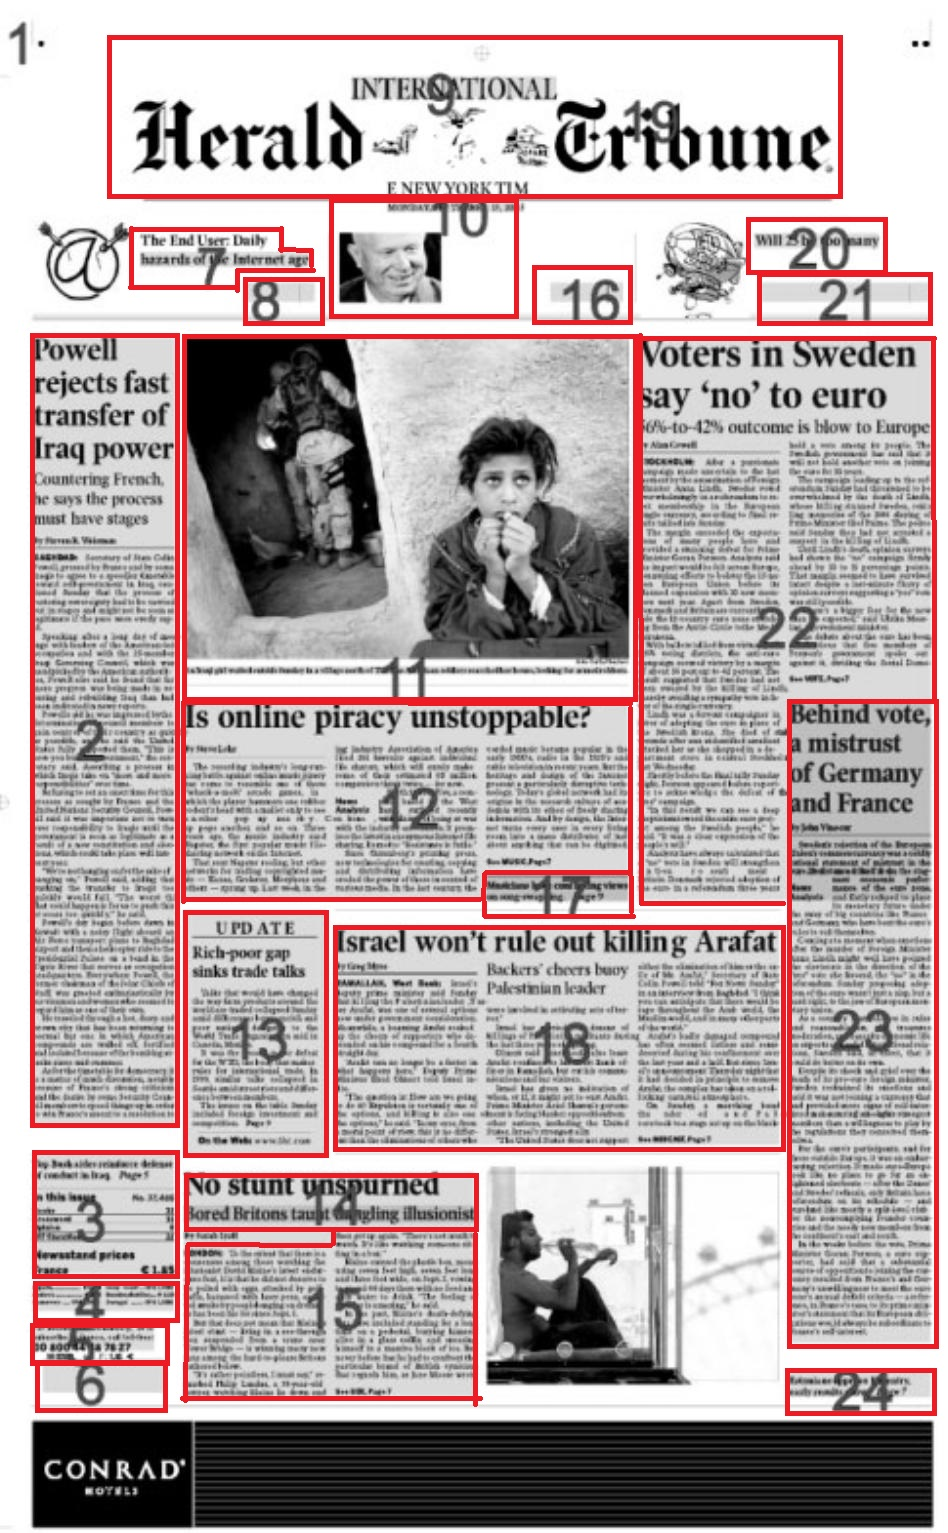
\includegraphics[width=0.5\linewidth]{img/tableDetection/readingOrder.jpg}
\caption{An example of layout analysis~\citep{hadjar2004xed}}
\label{fig:readingOrderExample}
\end{figure}

Various heuristics are being used for determining labels~\cite{logicalLayoutTemplate}. In the following list, we will be concerned with the few of the most widely used:

\begin{itemize}
\item[\emph{Templates}]

The most simple and basic approach is the technique of the already mentioned templates. It is based on a limited number of predefined document layouts (\emph{templates}), which already contain the information about the structure of individual elements. An input document is then matched to these layouts. Although a naive approach, in the OCR engines used widely for processing a single type of documents (such as ticket validation, recipe or passport recognition, recognition of forms filled out by patients in hospitals), this process yields almost perfect results.

\item[\emph{Rule-based approaches}]

A human reader often determines the logical succession of document elements by font settings and locations of the elements. Rule-based approaches take advantage of this fact and create heuristic \emph{rules} that determine the type of the element. For example, a rule for a page header could be "has the smallest y-axis value, has font size above 22pt, is bold, and is the only element on its line".

\item[\emph{Syntactic methods}]

These methods present the structure used for element labeling in a form of a set of formal (usually context free) grammars. These grammars contain rules for aggregating pixels into more structured entities until they form logical objects. Parsers for a syntactic analysis are automatically obtained from these grammars. They are then used to perform the actual labeling of the detected elements.

\item[\emph{Machine learning}]

Already mentioned in this thesis, a non-heuristic approach to logical layout analysis is the use of neural networks. Given enough information and time for training, the networks are able to determine the labeling on their own.

There exist various techniques of machine learning, distinguished by the way the neural networks are trained. For example, a neural network can be given a set of rules and input images, which leads the learning process to produce results similar to human observation. Also, it can be solely reliant on raw physical data and itself.

\end{itemize}

Worth mentioning are also techniques like \emph{Blackboard system} or \emph{Description language} or methods based on \emph{Hidden Markov Models}~\cite{logicalLayoutOther}.

Layout analysis is a crucial part of almost every OCR engine. If either geometric or logical layout analysis fails, the input of the recognition engine might contain corrupted data. This might lead to a significantly lower accuracy of the recognition process. 

In this thesis, our concern is not the headings and fonts, headers and footers of the image, as we focus solely on tabular data. However, this does not mean that layout analysis is unnecessary. We still need to extract the tables from page layout and ideally include also their headers, footers or any other information the table may contain.

\section{Table recognition}

The goal of table recognition is to determine if a table even is present on a page, and if yes, where and what its contents are. It is often divided into two parts --- \emph{table detection} and \emph{table decomposition}, with table detection determining the presence and placement of the table, and table decomposition analyzing the contents of the table and presenting a meaningful structure.

However, table detection often greatly depends on the decomposed structure of the table. For example, a table can be detected in the following way:

\begin{enumerate}
    \item find the individual lines (\emph{table decomposition})
    \item check which lines are aligned in a similar way (\emph{table detection})
    \item declare these lines to be in the same table (\emph{table decomposition})
    \item find different columns from the lines (\emph{table decomposition})
\end{enumerate}

If we were to first perform table detection and only then proceed to table decomposition, we would lose the important information about lines that we already obtained in step one. Therefore, many algorithms perform the table recognition process as a whole.

Extraction of table elements poses various difficulties. These are usually linked to the structure of a table. Although the extraction of elements of a simple $m{\times}n$ grid is an easy task achieved by a simple line detection algorithm (for example Hough transform), the missing presence of cell borders requires more complicated heuristics. Moreover, tables containing cells of different sizes, various numbers of cells in different rows, complicated headers or footers, multi-line cells and many more also require more complex solutions. We present a few of the possible obstacles in~\cref{fig:tableRecognitionObstacles}.

\begin{figure}[t]
\centering
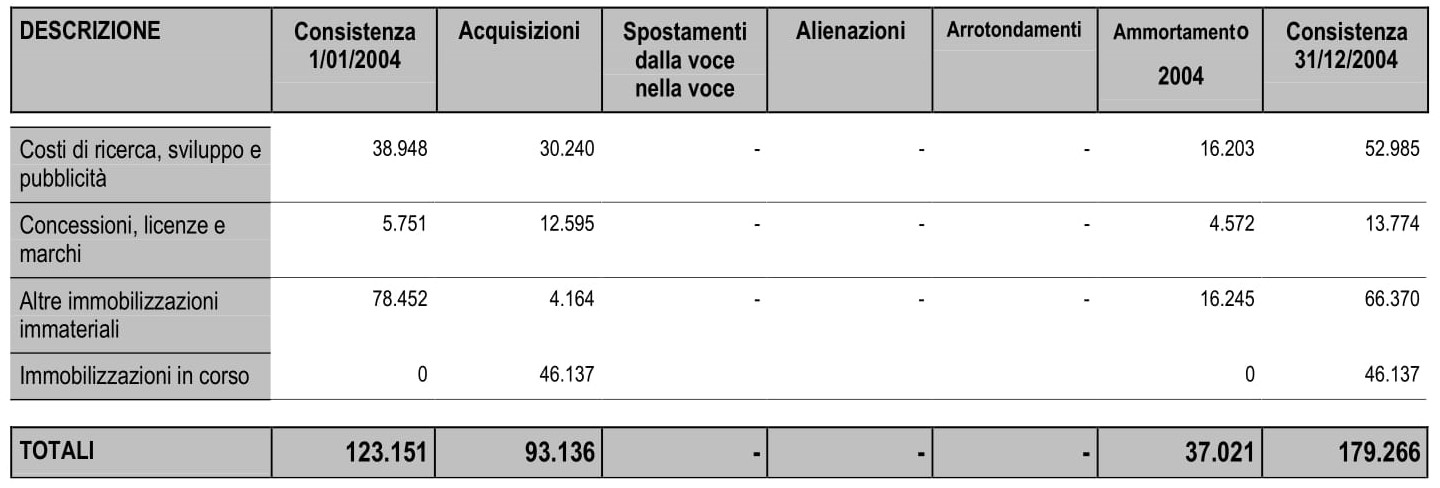
\includegraphics[width=0.7\linewidth]{img/tableDetection/recognitionProblematic.jpg}
\caption{A few of the basic problems with table recognition: missing horizontal and vertical lines; missing information in cells; multi-line cells in the first column and header row; different alignment of header and content cells }
\label{fig:tableRecognitionObstacles}
\end{figure}

In this section, we will overview some of the already existing table recognition algorithms. For the purposes of this thesis, we will specifically focus on the table recognition implementation of the Tesseract engine.

\subsection{Tesseract table recognition} \label{tableFind}

The Tesseract engine has been originally used solely for character detection. Over the years, however, many features have been added, including a table detection and recognition algorithm --- \emph{tablefind}.

Presented by~\citet{tableDetHeterogeneous}, the tablefind recognition algorithm is based on already existing Tesseract's features, including layout analysis (already mentioned in~\cref{sectionTessPageSegm}) and character detection (\cref{tesseractCharacterRecognition}). In this section, we will provide a brief overview of the algorithm, including its advantages and setbacks.

Following, we present the individual steps of the algorithm, along with their graphical interpretation in~\cref{fig:tesseractTableRecognition}: 

\begin{enumerate}
\item \emph{Layout analysis}

Layout analysis is performed by \emph{tab-stop detection} that is already included in the Tesseract library. We already mentioned this method in~\cref{sectionTessPageSegm}.

The results of this step, presented in~\cref{fig:tessTableDet1}, include not only a list of segmented blocks, but also the column layout and column partitions (sequences of connected components of the same type --- like text, image --- that do not cross any tab-line). The reason for this is the support for multi-column documents.

\item \emph{Column partition analysis}

The information about column layout and column partitions is next used to determine whether the column partition lies completely in one page column, or spans across multiple page columns. Analysis of column partition presence in table regions shows two major scenarios --- in the first case, table columns are reported as page columns, thereby destroying the columnar structure of a page. In the second case, table columns are ignored. We present the individual column partitions in~\cref{fig:tessTableDet2}.

\item \emph{Identifying table partitions}

The next step is to identify text column partitions that could possibly belong to a table --- \emph{table partitions}. This process is based on heuristics, by identifying partitions that have at least one large gap, consist of only one word, or overlap with other partitions along the y-axis.

This stage of the algorithm is performed quite aggressively, so although this process returns the desired table partitions, it also produces a lot of false alarms, like section headings, page headers, footers, equations and so on. A smoothing filter is applied to remove most of these unwanted partitions. However, as presented in~\cref{fig:tessTableDet3}, the presence of minor mistakes is not completely eliminated.

\item \emph{Detecting table columns}

Vertically aligned partitions are simply grouped into a single column with further removal of columns with only one partition, as presented in~\cref{fig:tessTableDet4}. This step pays a close attention to the page layout itself and tries to prevent merging two distinct columns, which is often an issue in full-page tables.

\item \emph{Creating tables}

The goal of the last step is to group table columns into a table. From the assumption that a flowing text does not share space with a table along the y-axis, boundaries of table columns are expanded to the page columns that contain them. Therefore, the within column table regions for each page column are obtained. When it comes to tables that span across multiple page columns, these are detected only if a table column exists that belong to both of these page columns.

\item \emph{Removal of false positives}

As the algorithm works quite aggressively, it produces a lot of false positives. Therefore, this step analyzes tables with only one column and removes those that do not suffice certain x-axis projection conditions. This produces the final result, presented in~\cref{fig:tessTableDet5}.

\end{enumerate}

The algorithm has been proved to have a 86\% precision. The biggest problems have shown to be full-page tables, often resulting in over or under-segmentation, partial detection or false positive detection~\citep{tableDetHeterogeneous}.

Another problem with tablefind is that currently, there exist no simple command that a user could run to see the output of this algorithm. To actually detect a table, a user must first write its own program where it uses the functions of the added Tesseract table recognition files. Then, he needs to process the data the library returns and output them in a meaningful format, which requires a non-trivial knowledge of the Tesseract implementation.

We will further present the results of this algorithm in~\cref{resultsTableFind}, where we compare them to our algorithm.
   
\begin{figure}[t]
\hspace*{\fill} 
\begin{subfigure}{0.31\textwidth}
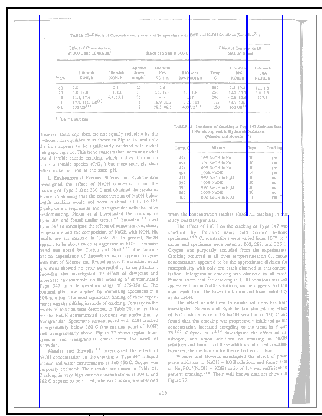
\includegraphics[width=\linewidth]{img/tableDetection/tableDetectionColumns.pdf}
\caption{Column layout}
\label{fig:tessTableDet1}
\end{subfigure}
\hspace*{\fill}
\begin{subfigure}{0.31\textwidth}
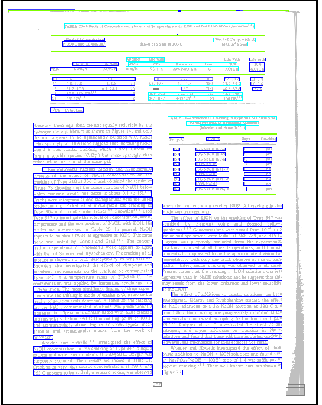
\includegraphics[width=\linewidth]{img/tableDetection/tableDetectionPartitions.pdf}
\caption{Column partitions}
\label{fig:tessTableDet2}
\end{subfigure}
\hspace*{\fill} 
\begin{subfigure}{0.31\textwidth}
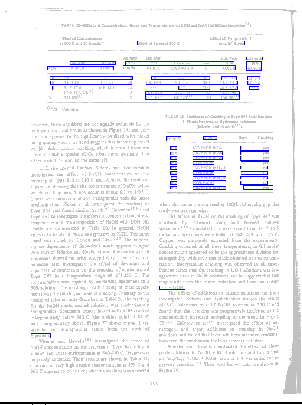
\includegraphics[width=\linewidth]{img/tableDetection/tableDetectionCandidate.pdf}
\caption{Candidate table partitions}
\label{fig:tessTableDet3}
\end{subfigure}
\hspace*{\fill}
\begin{subfigure}{0.31\textwidth}
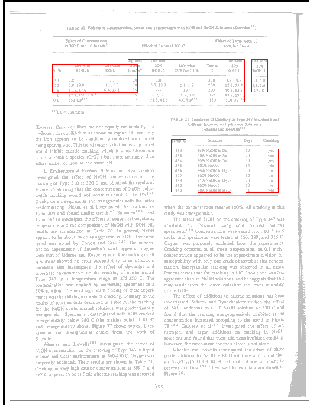
\includegraphics[width=\linewidth]{img/tableDetection/tableDetectionTabCols.pdf}
\caption{Table columns}
\label{fig:tessTableDet4}
\end{subfigure}
\begin{subfigure}{0.31\textwidth}
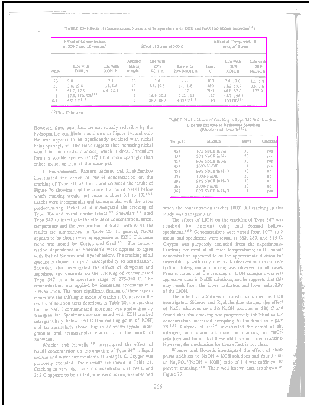
\includegraphics[width=\linewidth]{img/tableDetection/tableDetectionResult.pdf}
\caption{Detected table regions}
\label{fig:tessTableDet5}
\end{subfigure}
\caption{The process of Tesseract table recognition}
\label{fig:tesseractTableRecognition}
\end{figure}

\subsection{Other existing approaches}

Besides Tesseract, there exist heuristic approaches presented for table detection. In this section, we present an overview of a few of them and determine what they have in common, as well as point out their advantages and disadvantages.

Presented as one of the first table detection algorithms by~\citet{TRecs}, the \emph{T-Recs} table recognition system is based on a bottom-up approach of clustering word bounding boxes and building a "segmentation graph". This results in creating different regions of page. These are then evaluated according to certain criterion. If they satisfy them, the region is determined to be a table. Although widely used in the past, this techniques has a few setbacks. T-Recs is controlled by a set of numerical parameters, which result in different results of table detection depending on the layout that is given. These parameters need to be set manually. Moreover, it yields unsatisfactory results on multi-column documents.

Another algorithm was described by~\citet{MediumTable}. In single-column documents, a page can be easily segmented into individual text-lines. The table detection problem is then perceived as an optimization problem, where the start and end text-lines belonging to a table are identified by optimizing some quality function. However, this approach fails on multi-column documents, or on documents having more than one table.

\citet{tableDetectCesarini} describes another approach based on the document being hierarchically represented by a structure similar to a MXY tree. The presence of a table is determined by searching the tree for parallel lines, which contain white spaces and other perpendicular lines between them. Located tables can be merged on the basis of proximity and similarity criteria. However, this approach fails if no lines in tables are present --- which is usually the case of many tables.

Another method was presented by the \emph{pdf2table} project~\cite{pdf2table}. This method is based on assigning each text object of the page its positional attributes. Depending on them, text objects are then merged into single-lines (lines with only one text object), multi-lines (lines with more than one text object) and multi-line blocks (multiple multi-lines merged together). The table detection algorithm is based on merging multi-line blocks that may belong to the same table, with the help of a heuristic threshold that determines the greatest number of single-line objects between two multi-line blocks possible. This method also assumes the input to be a single-column document. However, a user can provide it with an information about the number of columns, which yields much more accurate results.

Multiple other approaches exist, each one of them working on different types of tables and yielding slightly different results. Worth mentioning is, for example, \emph{sparse line detection}~\cite{sparseLineDetection}, which already uses principles based on machine learning. Some of the other methods briefly mentioned by~\citet{otherDetection1} or~\citet{otherDetection2}.
